\documentclass{article}[18pt]
\usepackage{../../../../format}
\lhead{Software Engineering - Modelling and Analysis}

\begin{document}
\begin{center}
\underline{\huge The Role of Modelling}
\end{center}
\begin{defin}[Model]
	A model is something that provides an abstraction of a solution, capturing its essential characteristics and omitting unnecessary detail
\end{defin}
\begin{itemize}
	\item We use models to help produce solutions for both WSPs and also ISPs
\end{itemize}
\section{Why do we need to model?}
\begin{itemize}
	\item Complexity and size of software products means we need abstractions (models) to help predict how desired characteristics will be realised in the actual product
	\item So we use models to support such activities as:
	\begin{itemize}
		\item Requirements elicitation and specification
		\item Design of systems and applications
		\item Costing and planning
		\item Risk assessment
	\end{itemize}
	\item An important role for models in designing is that they help manage the cognitive load for large applications
\end{itemize}
\section{How do we develop a model}
\begin{itemize}
	\item Ideas about architecture can help with deciding what form of model we want to create
	\item Frameworks such as design patterns can help with organising the detailed structure of a model
\end{itemize}
\begin{important}[Models]
Creating models is an iterative process, we rarely get it right first time. It's a but like programming
\end{important}
\section{Perspectives and Viewpoints}
\begin{defin}[Perspective]
	Relates to a software development role. Each has their own set of interests and needs
\end{defin}

\begin{defin}[Viewpoint]
	A set of particular characteristics or attributes of a model, which in turn embody some specific aspect of software. A specific viewpoint is usually described by using one or more particular representations 
\end{defin}
\subsection{Design viewpoints}
\begin{itemize}
	\item An abstraction essentially "omits properties other than those of immediate interest"
	\item A viewpoint therefore focuses on a set of design attributes that relate to a particular abstraction
	\item The viewpoints we care about are:
	\begin{itemize}
		\item \textbf{Constructional} - Describing static properties and constructional details
		\item \textbf{Behavioural} - Describing the casual links between events and system responses
		\item \textbf{Functional} - describing the operations performed
		\item \textbf{Data modelling} - describing the forms of data elements and the relations between them
	\end{itemize}
\end{itemize}
\section{Software as an ISP}
\begin{center}
	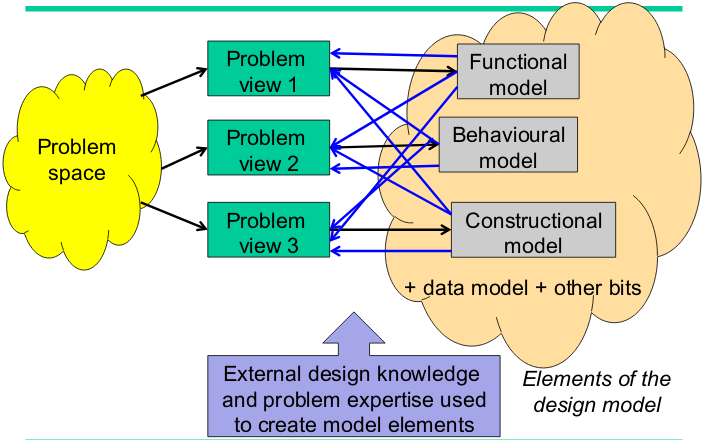
\includegraphics[scale=0.7]{ISP}
\end{center}
\section{Interconnectedness}
The viewpoints can be considered to be "projections" of the model, and are not independent
\section{Representations}
\begin{itemize}
	\item Provide the abstract descriptions we use in our models. A representation usually describes the attributes of the model that are related to a particular viewpoint
	\item Representations may use such forms as
	\begin{itemize}
		\item Textual
		\item Mathematical
		\item Diagrammatical
	\end{itemize}
\end{itemize}
They have many roles, such as:
\begin{itemize}
	\item Describing the characteristics and properties of the problem (usually for requirements analysis)
	\item Documenting the designer's ideas about the form of solution being proposed (for architectural design and construction)
	\item Explaining design ideas to others (customer, design team, implementers)
	\item Negotiating design ideas between team members (and possibly with the customer)
	\item Checking the degree of both consistency and completeness in a solution (V and V)
\end{itemize}
\subsection{Forms of representation}
Diagrams usually have a 'box and line' for and can be very informal. Established forms incorporate both:
\begin{itemize}
	\item Explicit semantics, provided by the symbols
	\item Implicit semantics, reflected by the 'conventions' adopted by users, such as positioning, orientation etc
\end{itemize}
The invisible nature of software also mean that there is no visual correspondence between a notation and the properties it intends to describe


\section{Abstraction}
\begin{itemize}
	\item A representation provides a particular abstraction of a system, related to the needs of a specific activity
	\item An abstraction omits the information that is not relevant to the task in hand, and emphasises the essential properties of interest
\end{itemize}
\section{Sketching}
Experts tend to sketch their designs, and often, they only formalise the diagrams if there is a specific requirement to do so\\
\\
In particular, they:
\begin{itemize}
	\item Rarely observe rules of diagram syntax very closely when sketching (if at all)
	\item Make notes, particularly when they recognise something which they know how to handle
	\item Make lists, often to help with checking that their model addresses necessary features
	\item Use the sketches to explore ideas, check consistency etc
\end{itemize}

\end{document}